%------------------------------------------------------------------------------
% Template file for the submission of papers to IUCr journals in LaTeX2e
% using the iucr document class
% Copyright 1999-2013 International Union of Crystallography
% Version 1.6 (28 March 2013)
%------------------------------------------------------------------------------

\documentclass[preprint]{iucr}              % DO NOT DELETE THIS LINE
\usepackage{siunitx}
\usepackage[utf8]{inputenc}
\usepackage{amsmath,amsfonts,amssymb}
%\usepackage[backend=biber]{biblatex}
\usepackage{graphicx}
\usepackage{cleveref}
\usepackage{algorithm2e}
\usepackage{xcolor}



    %-------------------------------------------------------------------------
     % Information about journal to which submitted
     %-------------------------------------------------------------------------
     \journalcode{S}              % Indicate the journal to which submitted
                                  %   A - Acta Crystallographica Section A
                                  %   B - Acta Crystallographica Section B
                                  %   C - Acta Crystallographica Section C
                                  %   D - Acta Crystallographica Section D
                                  %   E - Acta Crystallographica Section E
                                  %   F - Acta Crystallographica Section F
                                  %   J - Journal of Applied Crystallography
                                  %   M - IUCrJ
                                  %   S - Journal of Synchrotron Radiation

\begin{document}                  % DO NOT DELETE THIS LINE

     %-------------------------------------------------------------------------
     % The introductory (header) part of the paper
     %-------------------------------------------------------------------------

     % The title of the paper. Use \shorttitle to indicate an abbreviated title
     % for use in running heads (you will need to uncomment it).

\title{Single crystal diamond compound refractive lenses, in the lab and in the computer.}
%\shorttitle{Short Title}

     % Authors' names and addresses. Use \cauthor for the main (contact) author.
     % Use \author for all other authors. Use \aff for authors' affiliations.
     % Use lower-case letters in square brackets to link authors to their
     % affiliations; if there is only one affiliation address, remove the [a].

\cauthor[a]{Erik B}{Knudsen}{erkn@fysik.dtu.dk}{address if different from \aff}
\author[b]{Paw T}{Christiansen}
\author[a,c]{Steffen}{Sloth}
\author[d]{Xianbo}{Shi}
\aff[a]{Physics Dept., Techn. Univ. of Denmark, Fysikvej 307, DK-2800 Kgs. Lyngby, \country{Denmark}}
\aff[b]{JJ-Xray, Hørsholm,\country{Denmark}}
\aff[c]{3D-Imaging Centre, DTU, \country{Denmark}}
\aff[d]{Advanced Photon Source,\country{US}}

% Use \shortauthor to indicate an abbreviated author list for use in
     % running heads (you will need to uncomment it).

%\shortauthor{Soape, Author and Doe}

     % Use \vita if required to give biographical details (for authors of
     % invited review papers only). Uncomment it.

%\vita{Author's biography}

     % Keywords (required for Journal of Synchrotron Radiation only)
     % Use the \keyword macro for each word or phrase, e.g. 
     % \keyword{X-ray diffraction}\keyword{muscle}

\keyword{X-ray lens}\keyword{CRL}\keyword{simulation}




     % PDB and NDB reference codes for structures referenced in the article and
     % deposited with the Protein Data Bank and Nucleic Acids Database (Acta
     % Crystallographica Section D). Repeat for each separate structure e.g
     % \PDBref[dethiobiotin synthetase]{1byi} \NDBref[d(G$_4$CGC$_4$)]{ad0002}

%\PDBref[optional name]{refcode}
%\NDBref[optional name]{refcode}

\maketitle                        % DO NOT DELETE THIS LINE

\begin{synopsis}
Supply a synopsis of the paper for inclusion in the Table of Contents.
\end{synopsis}

\begin{abstract}
Abstract goes here.
\end{abstract}


     %-------------------------------------------------------------------------
     % The main body of the paper
     %-------------------------------------------------------------------------
     % Now enter the text of the document in multiple \section's, \subsection's
     % and \subsubsection's as required.

\section{Introduction}
%Describe the diamond CRL background - why do we care about this.
%1. High quality, durability
%2. Avoids the Be-problem (toxic)
%3. Low loss
Compound refractive Lenses (CRLs) have become an integral part of the optics toolbox for X-ray (and in a few experimental cases for neutron-) beamlines. Thus far though, the bread and butter CRL have been solely based on Beryllium technology. This is largely due to its low atomic number, and  hence low absorption. This performance comes with a number of drawbacks. First, the refractive index of Be is very close to 1 in most of the relevant spectrum, limiting the focusing power of the lens. Second, Be-lenses are generally made from Be-powder. This will inevitably generate Debye-scattering which may cause unwanted background in experiments. Third,  heat transport in Be is poor, which renders integration difficult when put in use in a high intensity environment. This can be nonetheless be done, but with effort. Fourth, Be is toxic and subject to restrictions wrt. handling. These latter points, coupled with a limited number of suppliers drives up the cost of such lenses significantly.

In recent times several groups\cite{otherDiamondLensPeople} have explored the possibility of shaping Diamond single crystals to x-ray lenses. Various modes of manufacturing have been explored including micromaching(?)\cite{waysToMakeDiamondLens} etc. In this work we explore the option of laser-ablation for "writing" lenses in single crystal diamond slabs. Using single crystals has the the advantage that scattering can be constrained to only few possible combinations of incoming and outgoing directions, which may be by construction guided into harmless places. (Also this avoids attenuating the beam by scattering)

Furthermore this process would allow JJ-Xray to make money.

\section{Methods}

\subsection{Laser writing  a lens}
In our chosen route toward practical diamond CRLs we have chosen to work with laser ablation\cref{fig:laser}. Here a laser pulse is focused onto a (presumably) flat diamond substrate. material from the substrate is vapourized(?) and transported away. By stepping a roughly Gaussian cross section laser beam across the substrate a shape is "written" with a line width approximately the same as the focused laser beam width. Depth resolution is created by writing in the same place repeatedly.\\
Something about how the laser can move across the surface.\\
Steffens laser ablation sims.\\
\begin{figure}
    \centering
    %\includegraphics{}
    \caption{The laser ablation process sketch}
    \label{fig:laser}
\end{figure}

Simulations of ablation here.
We need this if the article will be a sim only thing.



\subsection{Simulation}
To be able to assess in the future questions about the necessary resolution of written lens profiles we have build a simulation system within the Monte Carlo X-ray ray tracing software pcackage McXtrace\cite{BergbackKnudsen2013}. The idea is conceptually simple: Take a set of points representative of the lens profile, and directly put that into a model of the beamline under study and study the resulting beam profile at sample, or indeed go further and include also models of standard samples and/or data analysis procedures, to assess the effect of lens surface imperfections on the \emph{data} and conclusions thereof.

We have in this project developed a CRL-component for inclusion in the McXtrace package under the name \texttt{CRL\_measured\_profile}. Here an X-ray passes through the lens by means of the algorithm below (algorithm~\ref{alg:rayProp}).\\

%%% Coloring the comment as blue
\newcommand\mycommfont[1]{\footnotesize\ttfamily\textcolor{blue}{#1}}
\SetCommentSty{mycommfont}

\begin{algorithm}[H]
\label{alg:rayProp}
  Transport ray to lens entry plane\;
  \If{ray is within lens aperture}
  {
    calculate intersection with ideal parabolic profile\;
    propagate ray to the intersection point.\;
    \For{3 nearest data points/vertices}{
        \For{4 adjacent triangular patches $\Delta_i$}{ 
            $\mathbf{\tilde{n}} += \frac{1}{4} \mathbf{n_{\Delta i}}$
        }
        estimate the surface vertex normals at these vertices.(more details here)\;
    }
    interpolate surface at this point using the procedure of\cite{Nagata2005}.\;
    using partial differentials, get surface normal vector.\;
    update $\mathbf{k}$ to reflect inside material\;
    transport ray to second surface\;
    repeat loop above\;
    
  }
\end{algorithm}
\begin{figure}
    \centering
    %\includegraphics{}
    \caption{Sketch of the ray tracing process.}
    \label{fig:ray_trace_sketch}
\end{figure}

\begin{figure}
    \centering
    %\includegraphics{}
    \caption{Sketch of the interpolation process}
    \label{fig:interpol_sketch}
\end{figure}

Triangular surface patches generated how.

Looking ahead, the lens surface will be measured most conveniently in a regular rectangular grid. We should therefore make sure that our interpolation procedure is capapable of handling such data.Under the assumption that the beam will hit the   


\subsection{Measurement strategy}
PAW - tænker at du kan skrive her.


\section{Results}
\subsection{Sensofar et. al.}
\subsection{Simulations as done}
\begin{table}[]
    \centering
    \begin{tabular}{r|l}
        $\sigma_x$ & \SI{0.092}{mm} \\
        $\sigma_y$ & \SI{0.031}{mm} \\
        $\varepsilon_x$ & \SI{2.8e-6}{\radian mm}\\ 
        $\varepsilon_y$ & \SI{4.5e-8}{\radian mm}\\
        Ring Energy & \SI{7}{\giga \electronvolt}\\
        BM field strength & \SI{0.6}{\tesla}\\
    \end{tabular}
    \caption{Key beam parameters for the 1-BM-beamline at APS where measurements were performed.}
    \label{tab:beam_prms}
\end{table}

\begin{figure}
    \centering
    %\includegraphics{}
    \caption{Simulated beam characteristics at various points along the beam path}
    \label{fig:beamsims}
\end{figure}

\begin{figure}
    \centering
    %\includegraphics{}
    \caption{Sketch of the beamline including measuring points from above.}
    \label{fig:my_label}
\end{figure}

\subsection{Synch experiments}
Paw+Steffen

\section{Discussion}
\section{Outlook}


     % Appendices appear after the main body of the text. They are prefixed by
     % a single \appendix declaration, and are then structured just like the
     % body text.

\appendix
\section{Appendix title}

Text text text text text text text text text text text text text text
text text text text text text text.

\subsection{Title}

Text text text text text text text text text text text text text text
text text text text text text text.

\subsubsection{Title}

Text text text text text text text text text text text text text text
text text text text text text text.


     %-------------------------------------------------------------------------
     % The back matter of the paper - acknowledgements and references
     %-------------------------------------------------------------------------

     % Acknowledgements come after the appendices

\ack{Acknowledgements}

     % References are at the end of the document, between \begin{references}
     % and \end{references} tags. Each reference is in a \reference entry.

% \begin{references}
% \reference{Author, A. \& Author, B. (1984). \emph{Journal} \textbf{Vol}, 
% first page--last page.}
% \end{references}
\cite{knuth84}

%% Note added by Overleaf: If using bibtex, remove the "references" environment above, and uncomment the following line.
\referencelist{iucr}

     %-------------------------------------------------------------------------
     % TABLES AND FIGURES SHOULD BE INSERTED AFTER THE MAIN BODY OF THE TEXT
     %-------------------------------------------------------------------------

     % Simple tables should use the tabular environment according to this
     % model

\begin{table}
\caption{Caption to table}
\begin{tabular}{llcr}      % Alignment for each cell: l=left, c=center, r=right
 HEADING    & FOR        & EACH       & COLUMN     \\
\hline
     entry      & entry      & entry      & entry      \\
 entry      & entry      & entry      & entry      \\
 entry      & entry      & entry      & entry      \\
\end{tabular}
\end{table}

     % Postscript figures can be included with multiple figure blocks

\begin{figure}
\caption{Caption describing figure.}
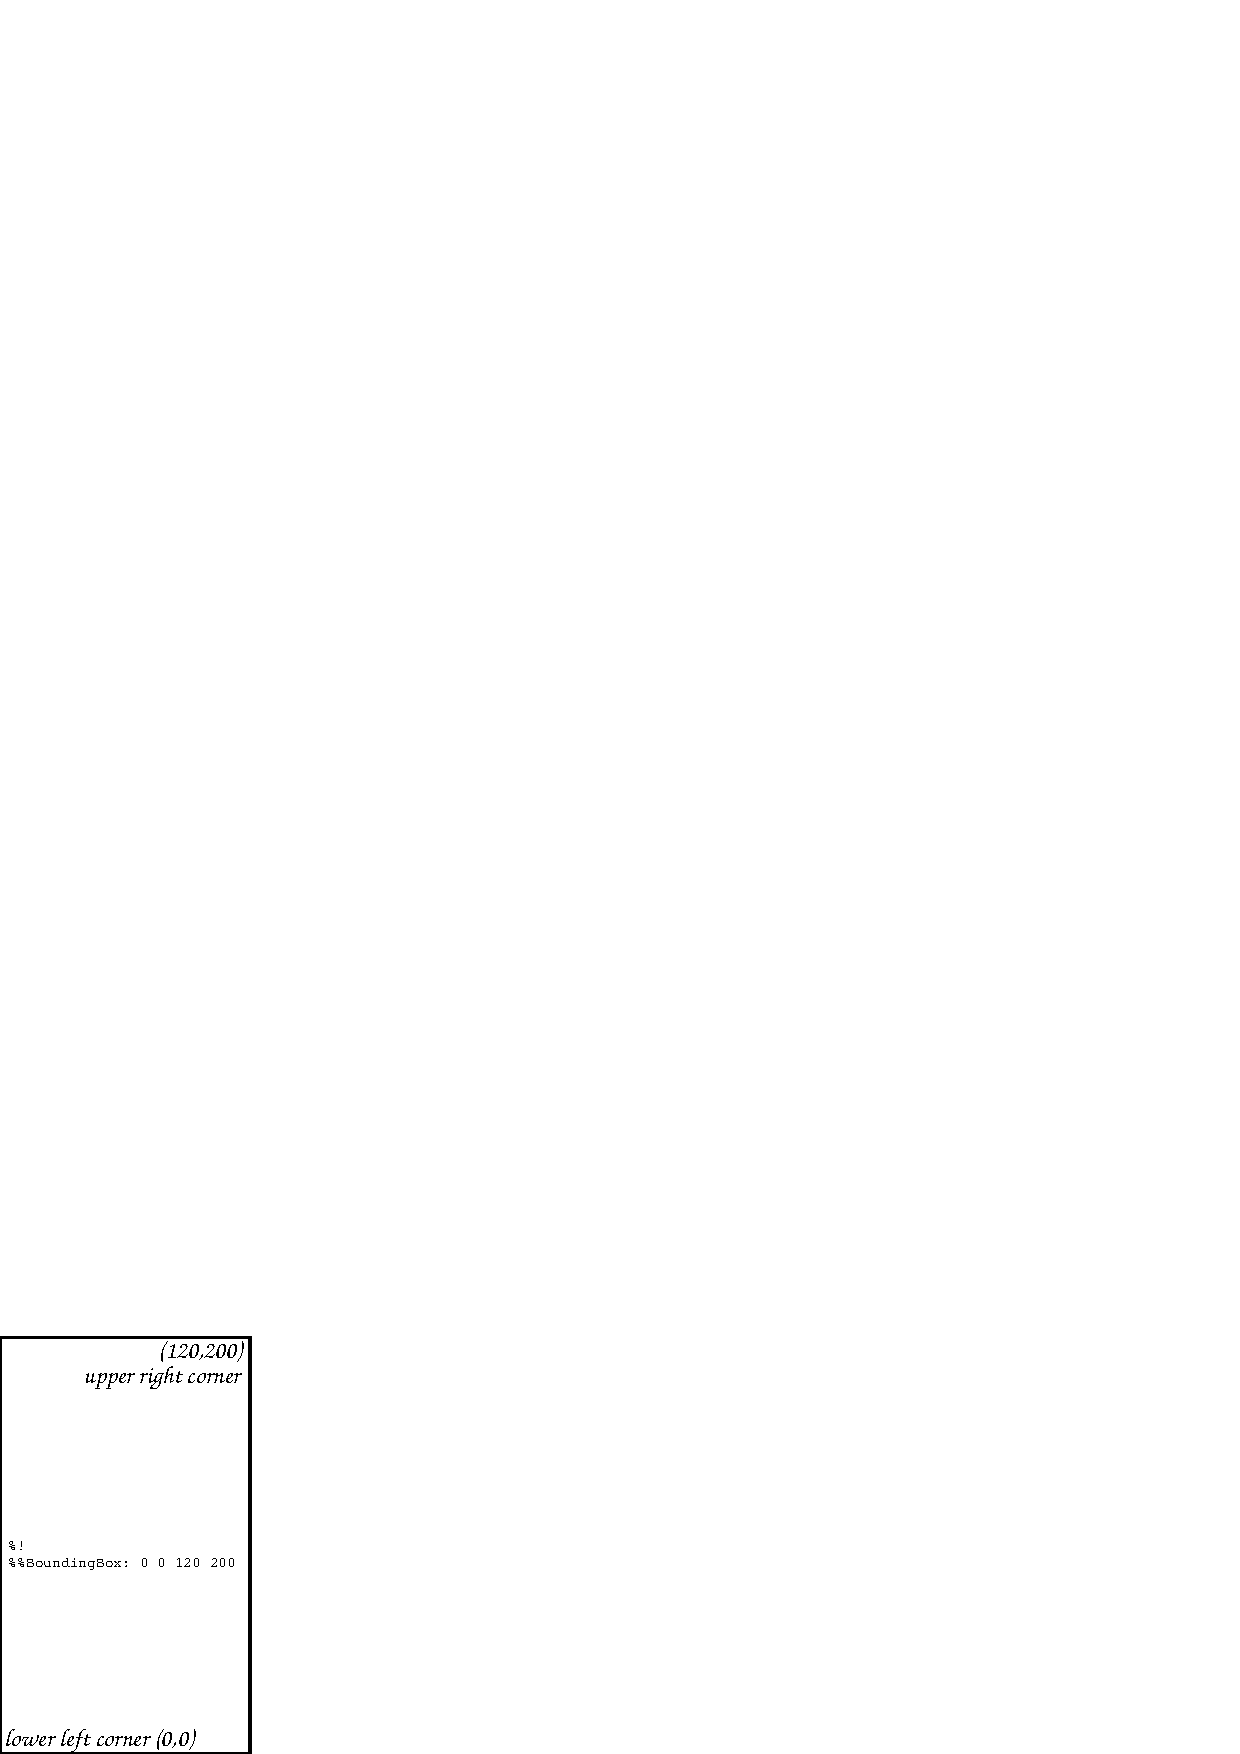
\includegraphics{fig1}
\end{figure}


\end{document}                    % DO NOT DELETE THIS LINE
%%%%%%%%%%%%%%%%%%%%%%%%%%%%%%%%%%%%%%%%%%%%%%%%%%%%%%%%%%%%%%%%%%%%%%%%%%%%%%
